\documentclass[11pt]{aghdpl}
\usepackage[english,polish]{babel}

\usepackage{polski}

\usepackage[utf8]{inputenc}


\usepackage{mathtools}
\usepackage{amsfonts}
\usepackage{amsmath}
\usepackage{amsthm}
\usepackage{tikz}
\usepackage{algorithm}
\usepackage{algorithmic}

\usepackage[
style=numeric,
sorting=none,
%
% Zastosuj styl wpisu bibliograficznego właściwy językowi publikacji.
language=autobib,
autolang=other,
% Zapisuj datę dostępu do strony WWW w formacie RRRR-MM-DD.
urldate=iso8601,
% Nie dodawaj numerów stron, na których występuje cytowanie.
backref=false,
% Podawaj ISBN.
isbn=true,
% Nie podawaj URL-i, o ile nie jest to konieczne.
url=false,
%
% Ustawienia związane z polskimi normami dla bibliografii.
maxbibnames=3,
% Jeżeli używamy BibTeXa:
backend=bibtex
]{biblatex}

\usepackage{csquotes}
% Ponieważ `csquotes` nie posiada polskiego stylu, można skorzystać z mocno zbliżonego stylu chorwackiego.
\DeclareQuoteAlias{croatian}{polish}

\addbibresource{bibliografia.bib}

% Nie wyświetlaj wybranych pól.
%\AtEveryBibitem{\clearfield{note}}


\usepackage{courier}

\usepackage{listings}
\lstloadlanguages{TeX}

\lstset{
	literate={ą}{{\k{a}}}1
           {ć}{{\'c}}1
           {ę}{{\k{e}}}1
           {ó}{{\'o}}1
           {ń}{{\'n}}1
           {ł}{{\l{}}}1
           {ś}{{\'s}}1
           {ź}{{\'z}}1
           {ż}{{\.z}}1
           {Ą}{{\k{A}}}1
           {Ć}{{\'C}}1
           {Ę}{{\k{E}}}1
           {Ó}{{\'O}}1
           {Ń}{{\'N}}1
           {Ł}{{\L{}}}1
           {Ś}{{\'S}}1
           {Ź}{{\'Z}}1
           {Ż}{{\.Z}}1,
	basicstyle=\footnotesize\ttfamily,
}

\AtBeginDocument{
	\renewcommand{\tablename}{Tabela}
	\renewcommand{\figurename}{Rys.}
}


\usepackage{array}
\usepackage{tabularx}
\usepackage{multirow}
\usepackage{booktabs}
\usepackage{makecell}
\usepackage[flushleft]{threeparttable}

\newcolumntype{C}[1]{>{\hsize=#1\hsize\centering\arraybackslash}X}


%---------------------------------------------------------------------------

\author{Wojciech Kumoń}
\shortauthor{W. Kumoń}

%\titlePL{Przygotowanie bardzo długiej i pasjonującej pracy dyplomowej w~systemie~\LaTeX}
%\titleEN{Preparation of a very long and fascinating bachelor or master thesis in \LaTeX}

\titlePL{Implementacja algorytmu weryfikacji modelowej własności LTL w środowisku rozproszonym}
\titleEN{Implementation of the distributed LTL model checking algorithm}


\shorttitlePL{Implementacja algorytmu weryfikacji modelowej własności LTL w środowisku rozproszonym}
\shorttitleEN{Implementation of the distributed LTL model checking algorithm}

\thesistype{Praca dyplomowa magisterska}

\supervisor{prof. dr hab. Marcin Szpyrka}
\degreeprogramme{Informatyka}
\date{2019}
\department{Katedra Informatyki Stosowanej}
\faculty{Wydział Elektrotechniki, Automatyki,\protect\\[-1mm] Informatyki i Inżynierii Biomedycznej}

\acknowledgements{Serdecznie dziękuję \dots tu ciąg dalszych podziękowań np. dla promotora, żony, sąsiada itp.}


\setlength{\cftsecnumwidth}{10mm}

\setcounter{secnumdepth}{4}
\brokenpenalty=10000\relax

\begin{document}

\titlepages

% Ponowne zdefiniowanie stylu `plain`, aby usunąć numer strony z pierwszej strony spisu treści i poszczególnych rozdziałów.
\fancypagestyle{plain}
{
	% Usuń nagłówek i stopkę
	\fancyhf{}
	% Usuń linie.
	\renewcommand{\headrulewidth}{0pt}
	\renewcommand{\footrulewidth}{0pt}
}

\setcounter{tocdepth}{2}
\tableofcontents
\clearpage

\chapter{Wstęp}

Weryfikacja modelowa to dziedzina umożliwiająca sprawdzenie systemu pod kątem specyfikacji.
Operacja taka jest zazwyczaj bardzo wymagająca pod kątem obliczeniowym, co skutkuje długimi czasami wykonania. Przeciwdziałać temu można na kilka sposobów, np. stosując uproszczenie modelu, czy wykorzystanie wydajniejszego procesora. Kolejna możliwość to stworzenie skalowanego systemu rozproszonego i właśnie ta metoda zostanie rozważona.

Samą specyfikację wyrazić można na wiele sposobów. W pracy wykorzystana zostanie logika LTL (ang. \textit{linear-time temporal logic}).


\section{Cel pracy}

Celem pracy jest implementacja rozproszonego algorytmu weryfikacji modelowej w oparciu o własności logiczne czasu liniowego - LTL dla języka Alvis z wykorzystaniem frameworka Spring.


\section{Struktura pracy}

W następnym rozdziale pracy omówione zostanie zagadnienie weryfikacji modelowej w kontekście tematu pracy.
Rozdział trzeci zawiera opis stworzonego rozwiązania.
W czwartym rozdziale znajduje się prezentacja uzyskanych wyników.
Piąty rozdział zawiera podsumowanie.

\chapter{Weryfikacja modelowa}

Systemy tworzone przez ludzi są coraz bardziej złożone oraz zwiększa się ich rola w życiu każdego z nas.
Błędy w oprogramowaniu skutkują stratami finansowymi, wizerunkowymi, opóźnieniami, a także utratą zdrowia i życia ludzi. Dowodzą temu następujące przykłady: nieudany start Ariane-5 (04.06.1996), błąd w procesorach Pentium II Intela, czy źle działająca maszyna do radioterapii, która spowodowała śmierć sześciu pacjentów w latach 1985-1987.


\section{Weryfikacja systemu}

Weryfikacja systemu ma na celu ustalenie, czy projekt posiada oczekiwane właściwości. Mogą one być dość podstawowe (np. nigdy nie dojdzie do zakleszczenia) lub związane z domeną (np. nie można wypłacić więcej pieniędzy, niż jest na koncie). Specyfikacja dostarcza informacji, jak system może oraz jak nie może się zachowywać. Oprogramowanie uważa się za poprawne, jeśli spełnia wszystkie właściwości. Schemat weryfikacji został przedstawiony na rys. \ref{fig:system_verification_scheme}.

\begin{figure}[h]
    \centering
    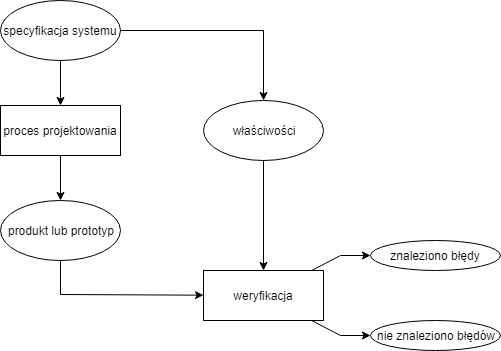
\includegraphics[height=8cm,keepaspectratio]{img/system_verification_schematic_view.png}
    \caption{Schemat tworzenia systemu wraz z jego weryfikacją (źródło~\cite{Bai08}).}
    \label{fig:system_verification_scheme}
\end{figure}

Podstawową formą radzenia sobie z tym problemem jest testowanie oprogramowania (testy jednostkowe, integracyjne, systemowe itp.). Polega ono na uruchamianiu kodu dla różnych ścieżek wykonania, po czym porównuje się ich wyjścia z oczekiwanymi. Niestety, przetestowanie wszystkiego okazuje się praktycznie niemożliwe, zwykle sprawdzane są jedynie warunki brzegowe (stanowi to mały podzbiór wszystkich kombinacji). 


\section{Weryfikacja modelowa}

Podczas tworzenia skomplikowanych systemów, kładzie się coraz większy nacisk na testowanie poprawności oprogramowania. Metody formalne mają duży potencjał na tym polu. Ich wczesna integracja (podczas procesu projektowania) dostarcza efektywnych technik weryfikacji.
Intuicyjnie, metody formalne można rozważać jako matematykę stosowaną dla modelowania i analizy systemów informatycznych. Zapewniają one poprawność z matematyczną dokładnością.

Techniki weryfikacji bazujące na modelu opisują zachowanie systemu deterministycznie i kompletnie. Samo tworzenie pełnego modelu może wykryć luki lub niespójności.
Po jego stworzeniu, wraz z otaczającymi algorytmami, następuje eksploracja stanów systemu.
Dzieje się to w podejściu ``brute-force`` - przejrzane zostają wszystkie możliwe scenariusze.
W ten sposób udowadnia się spełnialność właściwości. Weryfikacji dotyczy również kolejność zdarzeń w czasie, np. czy system zawsze odpowie na żądania klienta w tym samym porządku, w jakim je otrzymał.

\vspace{0.5cm}
\begin{figure}[h]
    \centering
    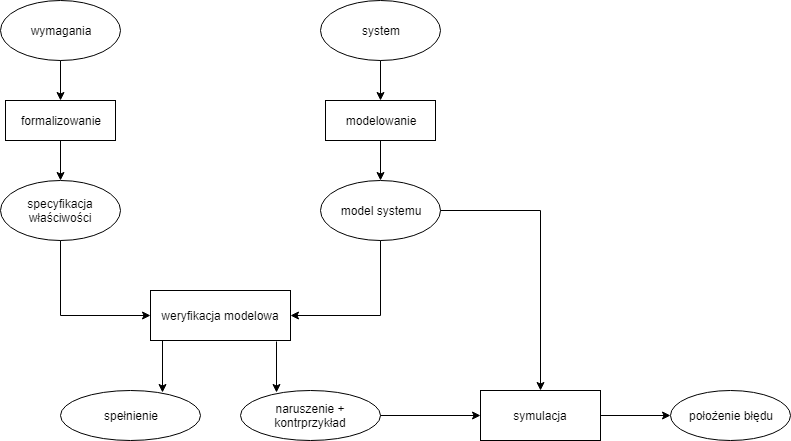
\includegraphics[width=\textwidth,keepaspectratio]{img/model_checking_approach_schematic_view.png}
    \caption{Schemat podejścia weryfikacji modelowej (źródło~\cite{Bai08}).}
    \label{fig:model_checking_scheme}
\end{figure}

Podejście to świetnie sprawdza się w wykrywaniu (częstych) błędów związanych z wielowątkowością. Typowe oczekiwane właściwości:
\begin{itemize}
\item osiągalność (niemożliwe jest zakleszczenie)
\item bezpieczeństwo (coś niepożądanego nigdy nie wystąpi \cite{Alp87})
\item żywotność (coś "dobrego" w końcu nastąpi \cite{Alp85})
\item uczciwość (czy przy odpowiednich warunkach zdarzenie występuje powtarzalnie)
\item właściwości czasu rzeczywistego
\end{itemize}

\vspace{0.5cm}
Model systemu zazwyczaj generuje się automatycznie z opisu w odpowiednim języku lub dialekcie wspieranym przez narzędzie. 
Weryfikator modelowy przeszukuje kolejne stany. Następnie sprawdzane są pod kątem właściwości. Po znalezieniu naruszenia, prezentowany zostaje kontrprzykład wraz z całą ścieżką wykonania, która do niego prowadzi. Pozwala to łatwo odtworzyć całą ścieżkę, a także znaleźć niespójność, która wymaga zmiany modelu (lub właściwości) - schemat na rys. \ref{fig:model_checking_scheme}.

\vspace{0.5cm}
\noindent
To nie jedyne zalety, kolejnymi mocnymi stronami weryfikacji modelowej są:
\begin{itemize}
\item To ogólna metoda weryfikacji, która sprawdza się zarówno przy tworzeniu oprogramowania, jak i projektowaniu sprzętu (np. procesorów).
\item Wspiera częściową weryfikację - możemy sprawdzać poszczególne właściwości niezależnie, nawet gdy pełna specyfikacja nie jest gotowa.
\item Wszystkie możliwości zostają sprawdzone.
\item Dostarcza informacji diagnostycznych po wykryciu niespełnionej właściwości.
\item Uruchomienie weryfikatora nie wymaga ekspertyzy na tym polu.
\item Łatwo zintegrować to rozwiązanie z cyklem wytwarzania oprogramowania.
\item Obecnie wzrasta zainteresowania tym podejściem.
\end{itemize}

\vspace{0.5cm}
\noindent
Oczywiście nie brak także wad:
\begin{itemize}
\item Weryfikowany jest model systemu, a nie sam system. Brak tu gwarancji, że implementacja poprawnie go odtwarza.
\item Sprawdzane są tylko wykorzystane wymagania. Nie można wnioskować o poprawności właściwości, które nie zostały sprawdzone (błąd niedokładnej specyfikacji \cite{Lam05}).
\item Aplikacje oparte na dużej ilości danych mogą posiadać zbyt wiele stanów, aby je wszystkie wygenerować, a nawet ich liczba może być nieskończona.
\item Podatność na problem eksplozji przestrzeni stanów \cite{Cla11}.
\end{itemize}


\section{Logika LTL}

Logika LTL to jednak z logik temporalnych. Opiera się na liniowej strukturze czasu.
Jej składnia i semantyka pozwala precyzyjnie opisywać bogate spektrum właściwości systemu, włączając w to m.in bezpieczeństwo czy żywotność \cite{Bel17}.
``Temporalna`` oznacza umiejscawianie zdarzeń relatywnie względem innych, to pewna abstrakcja ponad czasem.  Z tego powodu niewykonalne jest sprawdzenie, czy maksymalne opóźnienie między zdarzeniami wynosi $500ms$.

Formuły LTL ponad zbiorem $AP$ wyrażeń atomowych przedstawia poniższa gramatyka:
\begin{gather}
\varphi::= true \,\, | \,\, false \,\, | \,\, a \,\, | \,\, \neg\varphi \,\, | \,\, \varphi \land \psi \,\, | \,\, \varphi \lor \psi \,\, | \,\, \varphi \Rightarrow \psi \,\, | \,\, \varphi \Leftrightarrow \psi \,\, | \nonumber\\
\mathbf{X}\varphi \,\, | \,\, \mathbf{F}\varphi \,\, | \,\, \mathbf{G}\varphi \,\, | \,\, \varphi\mathbf{U}\psi \,\, | \,\, (\varphi)\nonumber
\end{gather}
gdzie $a \in AP$ \\
Wyjaśnienie symboli (intuicyjna semantyka przedstawiona jest na rys. \ref{fig:ltl_semantics}): \\
$\mathbf{X}$ - $ne\mathbf{X}t$ - w następnym stanie \\
$\mathbf{U}$ - $\mathbf{U}ntil$ - aż do pewnego momentu w przyszłości \\
$\mathbf{F}$ - $\mathbf{F}inally$ - teraz lub w przyszłości \\
$\mathbf{G}$ - $\mathbf{G}lobally$ - teraz i w każdym momencie w przyszłości
\vspace{0.5cm}

\begin{figure}[h]
    \centering
    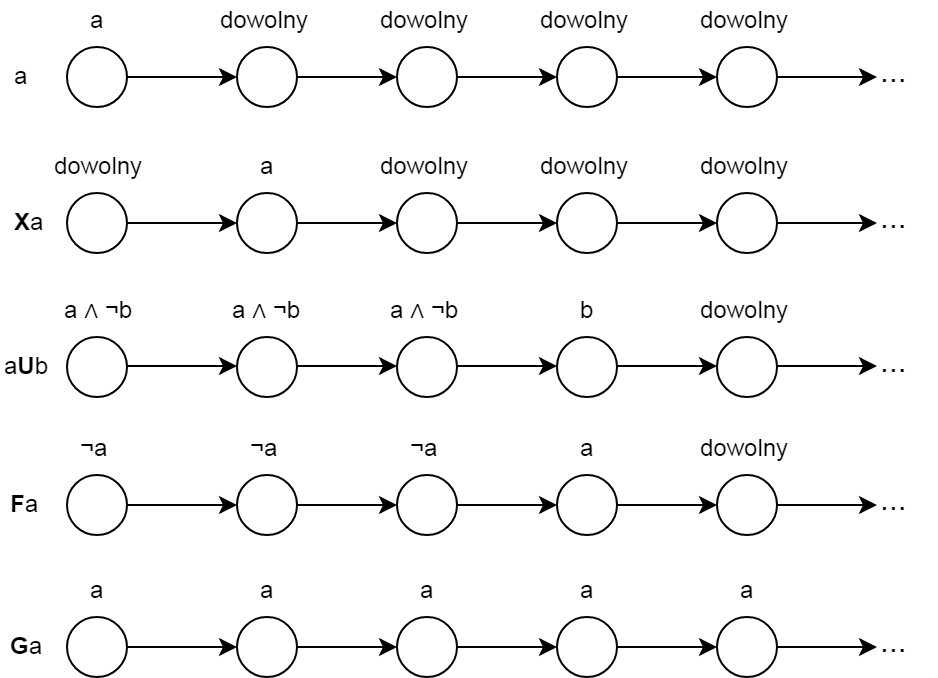
\includegraphics[height=11cm,keepaspectratio]{img/ltl_intuitive_semantics.png}
    \caption{Intuicyjna semantyka temporalnych modalności (źródło~\cite{Bai08}).}
    \label{fig:ltl_semantics}
\end{figure}

Przykładowe formuły LTL:
\begin{itemize}
\item $\mathbf{G}\neg\varphi$ - niemożliwe jest osiągnięcie stanu posiadającego $\varphi$ (bezpieczeństwo)
\item $\mathbf{G}(\varphi\Rightarrow\mathbf{F}\psi)$ - dla dowolnego stanu, jeśli posiada on $\varphi$, w końcu znajdziemy stan posiadający $\psi$ (żywotność)
\item $\mathbf{FG}\varphi$ - w końcu znajdziemy taki stan, od które zawsze spełnione będzie $\varphi$ (stabilność)
\end{itemize}


\section{Automat Büchiego}

W poprzedniej sekcji przedstawiona została liniowa logika LTL.
Niestety w obecnej postaci nie można jej wykorzystać do weryfikacji modelowej.
Punktem startowym jest system tranzycyjny $TS$ oraz formuła LTL $\varphi$, która formalizuje wymaganie dla $TS$.
Zadanie polega na sprawdzeniu, czy $TS \models \varphi$.
Jeśli $\varphi$ jest naruszona, szczegóły błędy powinny zostać dostarczone w celu jego naprawienia.
Manualne dowodzenie $TS \models \varphi$ to zazwyczaj bardzo trudny proces (zwykle systemy tranzycyjne są ogromne).
Dodatkowo rzadkim przypadkiem jest jedna formuła do weryfikacji.
Wymagania składają się na ich zbiór, taki jak $\varphi_1,...,\varphi_k$.
Wynikają z tego dwie opcje - można połączyć je w jedną $\varphi_1 \land ... \land \varphi_k$, aby uzyskać specyfikację wszystkich wymagań naraz lub traktować każde wymaganie $\varphi_i$ niezależnie.
Drugie podejście często okazuje się wydajniejsze.
Ponadto znalezienie błędu podczas sprawdzania pełnej specyfikacji nie dostarcza tak precyzyjnych danych diagnostycznych.

Pomiędzy logiką temporalną a teorią $\omega$-regularnych języków zachodzi bliska relacja \cite{Sis83}\cite{Wol83}.
Języki $\omega$-regularne są analogiczne do regularnych, lecz są zdefiniowane na nieskończonych słowach (zamiast skończonych).
Rozpoznawane są one przez automat Büchiego \cite{Buch66}.
To skończony automat, który operuje na nieskończonych słowach.
Nieskończone słowo jest akceptowane przez automat Büchiego wtedy i tylko wtedy, gdy stan akceptujący wystąpi nieskończenie wiele razy \cite{Sis87}.
Formalnie, deterministyczny automat Büchiego to krotka $A = (Q,\Sigma,\delta,q_0,F)$ składająca się z następujących elementów:
\begin{itemize}
\item $Q$ - skończony zbiór. Elementy $Q$ nazywane są stanami $A$.
\item $\Sigma$ - skończony zbiór nazywany alfabetem.
\item $\delta: Q \times \Sigma \rightarrow Q$ - funkcja nazywana funkcją tranzycji $A$.
\item $q_0$ - element $Q$, nazywany stanem początkowym $A$
\item $F \subseteq Q$ - warunek akceptujący. $A$ akceptuje dokładnie takie przejścia, gdzie przynajmniej jeden z nieskończenie często występujących stanów jest w $F$.
\end{itemize}
W niedeterministycznym automacie Büchiego (NBA - ang. \textit{non-deterministic Büchi automaton}), funkcja tranzycji $\delta$ zastąpiona jest relacją tranzycji $\Delta$, która zwraca zbiór stanów, a w miejscu stanu początkowego $q_0$ znajduje się zbiór stanów początkowych.

Uogólniony automat Büchiego (GBA - ang. \textit{generalized Büchi automaton}), to krotka $A = (Q,\Sigma,L,\Delta,Q_0,F)$:
\begin{itemize}
\item $Q$ - skończony zbiór. Elementy $Q$ nazywane są stanami $A$.
\item $\Sigma$ - skończony zbiór nazywany alfabetem.
\item $\delta: Q \times \Sigma \rightarrow 2^Q$ - funkcja nazywana funkcją tranzycji $A$.
\item $Q_0$ - podzbiór $Q$, nazywany stanami początkowymi
\item $F$ - warunek akceptujący. Składa się z zera lub więcej akceptujących zbiorów. Każdy taki zbiór $F_i \in F$ jest podzbiorem $Q$.
\end{itemize}
Pomimo różnic, GBA to ekwiwalent NBA w kategorii siły ekspresji.
W związku z tym możliwa jest jego konwersja do NBA \cite{Mer14}\cite{Dol95}.

Na rys. \ref{fig:nba1} oraz \ref{fig:nba2} znajdują się przykładowe NBA, wraz z odpowiadającymi im formułami.

\begin{figure}[h]
    \centering
    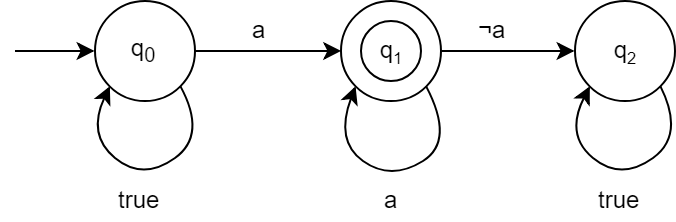
\includegraphics[width=8cm,keepaspectratio]{img/nba1.png}
    \caption{NBA dla $\mathbf{FG}a$ (źródło~\cite{Bai08}).}
    \label{fig:nba1}
\end{figure}
\begin{figure}[h]
    \centering
    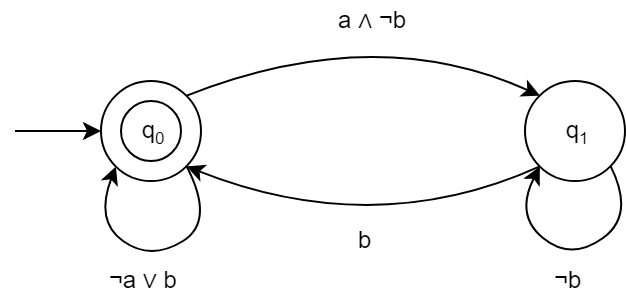
\includegraphics[width=8cm,keepaspectratio]{img/nba2.png}
    \caption{NBA dla $\mathbf{G}(a \Rightarrow \mathbf{F}b)$ (źródło~\cite{Bai08}).}
    \label{fig:nba2}
\end{figure}

\noindent
Algorytm weryfikacji formuły LTL $\varphi$ w systemie tranzycyjnym $TS$ wygląda następująco:
\begin{enumerate}
    \item Zaneguj formułę $\varphi$ otrzymując $\neg\varphi$.
    \item Skonstruuj niedeterministyczny automat Büchiego $A_{\neg\varphi}$ odpowiadający formule $\neg\varphi$.
    \item Skonstruuj wynikowy system tranzycyjny $TS \otimes A$.
    \item Jeśli istnieje ścieżka $\pi$ w $TS \otimes A$ spełniająca akceptujący warunek $A$, zwróć ``nie`` wraz z opisem ścieżki $\pi$, w przeciwnym razie zwróć ``tak``.
\end{enumerate}

Sam schemat przedstawiający jak działa weryfikacja modelowa, kiedy wykorzystujemy logikę LTL do opisu właściwości, znajduje się na rys. \ref{fig:ltl_model_checking}.

\begin{figure}[h]
    \centering
    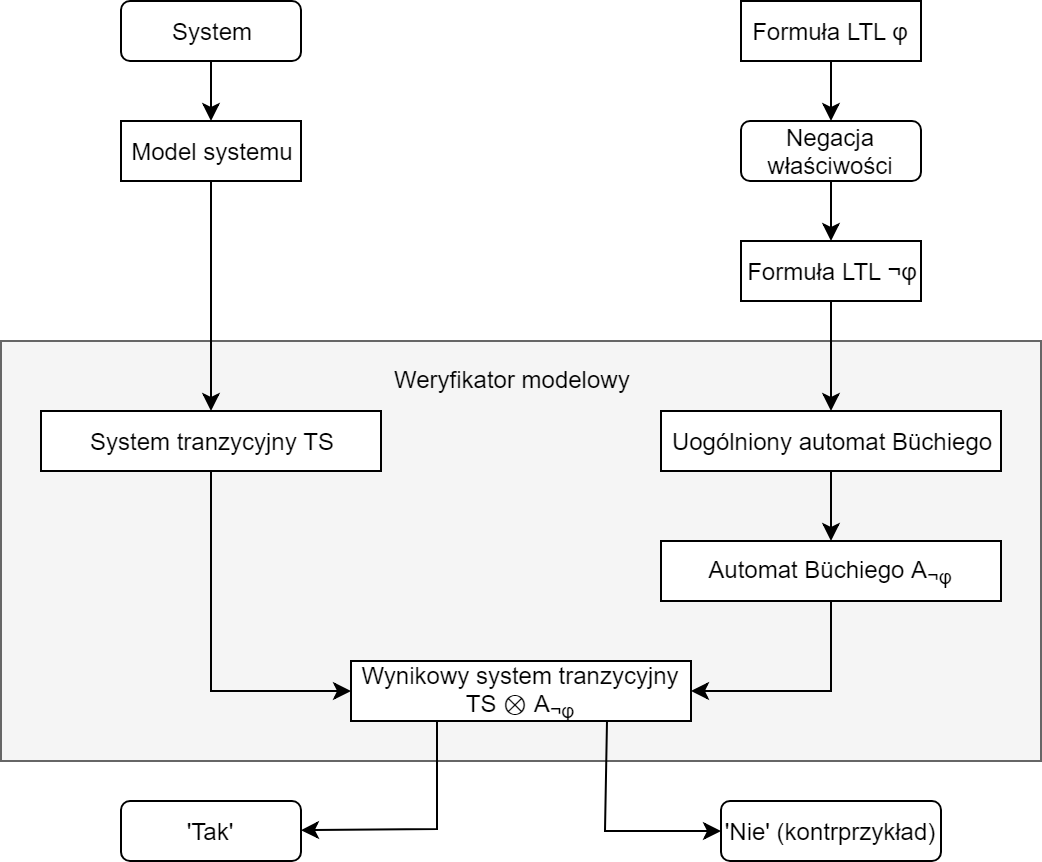
\includegraphics[height=11cm,keepaspectratio]{img/ltl_model_checking_overview.png}
    \caption{Przegląd weryfikacji modelowej LTL (źródło~\cite{Bai08}).}
    \label{fig:ltl_model_checking}
\end{figure}


\section{Eksploracja stanów systemu}

Posiadanie modelu systemu nie oznacza dostępności pełnego grafu stanów.
Może to być niepraktyczne lub nawet niemożliwe ze względu na liczbę stanów.
Preferowanym podejście to generowanie kolejnych stanów i ich weryfikacja ich w locie.
Takie rozwiązanie pozwala na wykrycie niespójności we wczesnym etapie, unikając generacji całej przestrzeni stanów.

Kolejnym czynnikiem wpływającym na wydajność jest sam algorytm budujący graf stanów.
W przypadku skomplikowanych systemów spodziewać się można olbrzymiego grafu, więc również czas jego tworzenia będzie odzwierciedlał rozmiar.
Moc obliczeniowa jednego procesora może okazać się niewystarczająca.
Warto więc wykorzystać algorytmy równoległe.
Standardowym rozwiązanie to DFS (przeszukiwanie w głąb - ang. \textit{Depth-first search}) \cite{God94}\cite{Hol99}.
Występuje w wielu wersjach mających zwiększyć jego wydajność.
Z czasem powstała też nowa grupa algorytmów.
Opiera się na podziale grafu na silnie spójne składowe, wywodzi się ona z algorytmu Tarjana \cite{Jac05}.
Złożoność obliczeniowa tych algorytmów jest liniowa $O(m + n)$, gdzie $m$ to liczba krawędzi, a $n$ oznacza ilość stanów.
Wszystkie korzystają z tej samej zasady eksploracji - przeszukiwania wstecznego (ang. \textit{post-order}).
Faktem jest, że problem takiego przeszukiwania jest P-zupełny, więc skalowany, równoległy algorytm tego typu najprawdopodobniej nie istnieje \cite{Reif85}.

Algorytmem wartym uwagi jest \textit{on-the-fly OWCTY algorithm} \cite{Bar12}.
Opiera on się na algorytmie OWCTY (ang. \textit{One Way Catch Them Young}) \cite{Cer03} oraz MAP (ang. \textit{Maximal Accepting Predecessor}) \cite{Bri04}.
Co więcej, pozwala na zrównoleglenie obliczeń.

\chapter{Architektura systemu}

Założeniem projektu było stworzenie algorytmu weryfikacji modelowej w oparciu o własności LTL dla języka Alvis w środowisku rozproszonym.

Alvis to język formalny, którego celem jest dostarczenie elastyczności w modelowaniu systemów współbieżnych i czasu rzeczywistego wraz z możliwością weryfikacji opartej o metody formalne.
Stanowi połączenie zalet języków wysokiego poziomu z graficznym budowaniem zależności między podsystemami (nazywanymi agentami).
% TODO jak dużo o Alvisie takiego wstępu?


\section{System rozproszony}

Architektura systemu została zaplanowana tak, aby wydzielić funkcjonalności do odseparowanych aplikacji.
Całość składa się z 3 programów oraz bazy danych.
Jej schemat ogólny został przedstawiony na rys. \ref{fig:system_overview}.

\begin{figure}[h]
    \centering
    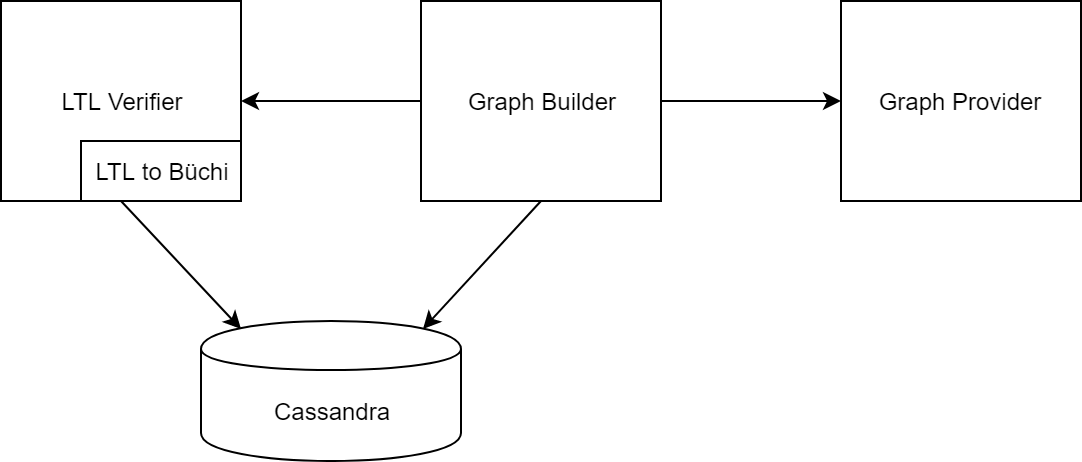
\includegraphics[width=\linewidth,keepaspectratio]{img/system_overview.png}
    \caption{Schemat ogólny systemu.}
    \label{fig:system_overview}
\end{figure}

Pierwszym elementem jest \textit{Graph Provider} (\textbf{GP}).
Spełnia on dwa zadania.
Pierwsze z nich to dostarczanie wszystkich osiągalnych tranzycji dla danego stanu.
Drugie umożliwia otrzymanie stanów dla zadanej tranzycji, które można odwiedzić z wybranego stanu źródłowego.
Serwis ten enkapsuluje działanie całej domeny.
Jako jedyny dostarcza dane, dzięki którym da się zbudować całą przestrzeń stanów.
GP spełnia prosty interfejs przedstawiony w listingu \ref{lst:graph_provider_interface}.

\begin{lstlisting}[caption={Interfejs implementowany przez GP.},captionpos=b,label={lst:graph_provider_interface}]
    public interface GraphProvider {
        Collection<Transition> allTransitionFromState(SystemState from);

        Collection<SystemState> allReachableStates(SystemState from,
                                                   Transition through);
    }
\end{lstlisting}

\textit{LTL Verifier} (\textbf{LV}) to główna serwerowa aplikacja zajmująca się weryfikacją modelową i zawiera główną część tego algorytmu.
Konwertuje ona także formuły LTL do automatów Büchiego.
Napisana została w języku Java z wykorzystaniem frameworka Spring.
Interfejs implementowany przez LV opisuje listing \ref{lst:ltl_verifier_interface}.

\begin{lstlisting}[caption={Interfejs implementowany przez LV.},captionpos=b,label={lst:ltl_verifier_interface}]
    public interface LtlVerifier {
        public VerificationJobId createVerificationJob(List<State> initialStates);

        public VerificationResult newStates(NewStates newStates,
                                            VerificationJobId id);

        public VerificationResult finish(VerificationJobId id);
    }
\end{lstlisting}

\textit{Graph Builder} (\textbf{GB}) spełnia rolę serca systemu.
To centrum sterowania, które inicjuje zapytania do pozostałych aplikacji.
Zarządza eksploracją kolejnych stanów, a także wysyła je do weryfikacji.
Zarówno GB jak i LV komunikują się z bazą danych (Cassandra), aby czytać i zapisywać stany czy tranzycje.
Komunikacja między GB a GP zachodzi za pomocą Apache Thrift, wykorzystując binarny protokół przesyłając dane siecią.
Zapytania GB do LV realizowane są poprzez protokół HTTP w formacie JSON.

% TODO dopisać o celach i możliwościach architektury, może diagram z wyszczególnionymi protokołami komunikacji

\chapter{Algorytm weryfikacji}

Zastosowany algorytm weryfikacji modelowej opiera się głównie na \textit{on-the-fly OWCTY} \cite{Bar12}, który został dostosowany do wykorzystania w środowisku rozproszonym.

\begin{algorithm}
\caption{$ detectAcceptingCycle() $}
\label{alg:detectAcceptingCycle}
\begin{algorithmic}[1]
\REQUIRE $ G = (V,E,ACC) $

\STATE $ initialStates \leftarrow getInitialStates() $
\STATE $ approximationSet \leftarrow initialise(initialStates) $
\STATE $ oldSize \leftarrow \infty $
\WHILE{$ (approximationSet.size \neq oldSize)\ \mathbf{and}\ (approximationSet.size > 0) $}
  \STATE $ oldSize \leftarrow approximationSet.size $
  \STATE $ eliminateNoAccepting(approximationSet) $
  \STATE $ eliminateNoPredecessors(approximationSet) $
\ENDWHILE
\RETURN $ approximationSet.size > 0 $
\end{algorithmic}
\end{algorithm}

Algorytm OWCTY wykorzystuje sortowanie topologiczne dla detekcji cykli.
Zapewnia liniową złożoność czasową przy jednoczesnym uniknięciu przeszukiwania w głąb, co umożliwia wykonanie równoległe.
Niestety procedura sortowania topologicznego nie może bezpośrednio wykryć cykli akceptujących.
Zamiast tego wykorzystuje się eliminację cykli nieakceptujących.
Obliczany jest zbiór stanów poprzedzanych przez cykl akceptujący (\textit{approximationSet}).
Jeśli po zakończeniu algorytmu zbiór ten jest pusty, nie ma cyklu akceptującego.
Sam zbiór wylicza się w kilku fazach.
Pierwsza z nich, czyli \textit{initialise()} (algorytm \ref{alg:initialise}) eksploruje pełną przestrzeń stanów systemu oraz przygotowuje niezbędne dane dla kolejnych faz.
Kolejne dwie usuwają ze zbioru stany, które nie mogą być częścia cyklu akceptującego.

Jedna z nich to \textit{eliminateNoAccepting()} (algorytm \ref{alg:eliminateNoAccepting}).
Zaczyna się od pozostawienia w zbiorze jedynie stanów akceptujących (linie 3-10).
Następnie obliczane są wartości liczby poprzedników dla każdego wierzchołka.
To część procedury osiągalności, która poszerza cały zbiór, a ten może zawierać już nie tylko stany akceptujące (linie 11-22).

Ostatnia faza OWCTY to \textit{eliminateNoPredecessors()} (algorytm \ref{alg:eliminateNoPredecessors}).
Bazuje ona na sortowaniu topologicznym.
Wykorzystuje liczbę poprzedników wyliczonych w \textit{eliminateNoAccepting()}, aby iteracyjnie usuwać wierzchołki ze zbioru, kiedy ich stopień (w podgrafie tworzonym przez stany pozostałe w zbiorze) równy jest 0.
Kiedy wierzchołek znika ze zbioru, należy zmniejszyć stopień jego następników o 1.
Brak takich następników oznacza zakończenie fazy.
\textit{EliminateNoAccepting()} oraz \textit{eliminateNoPredecessors()} wykonywane są w pętli, dopóki zachodzą jakieś zmiany.

Opis użytych zmiennych/procedur w algorytmach \ref{alg:detectAcceptingCycle} i \ref{alg:initialise}:
\begin{itemize}
\item $ G = (V,E,ACC) $ - wejściowy graf składający się ze zbiorów wierzchołków, krawędzi i stanów akceptujących
\item \textit{getInitialStates()} - procedura zwracająca zbiór stanów początkowych dla grafu $G$
\item \textit{isAccepting(x)} - zwraca prawdę, jeśli stan $x$ jest akceptujący, fałsz w przeciwnym wypadku
\item \textit{acceptingCycleFound()} - służy do wcześniejszego zakończenia algorytmu (kiedy cykl akceptujący został wykryty bez eksploracji całej przestrzeni stanów)
\end{itemize}

\begin{algorithm}
\caption{$ initialise(initialStates) $}
\label{alg:initialise}
\begin{algorithmic}[1]
\REQUIRE $ initialStates $

\STATE $ approximationSet \leftarrow initialStates $
\STATE $ q \leftarrow new\ Queue() $
\STATE $ q.pushBack(initialStates) $
\WHILE{$ q.isNotEmpty() $}
  \STATE $ s \leftarrow q.popFront() $
  \FORALL{$ t \in getSuccessors(s) $}
    \IF{$ t \notin approximationSet $}
      \STATE $ approximationSet.add(t) $
      \STATE $ q.pushBack(t) $
    \ENDIF
    \IF{$ isAccepting(t) $}
      \IF{$ (t == s)\ \mathbf{or}\ (approximationSet.getMap(s) == t) $}
        \STATE $ acceptingCycleFound() $
        \RETURN
      \ENDIF
      \STATE $ approximationSet.setMap(t, max(t, approximationSet.getMap(s))) $
    \ELSE
      \STATE $ approximationSet.setMap(t, approximationSet.getMap(s)) $
    \ENDIF
  \ENDFOR
\ENDWHILE
\RETURN $ approximationSet $
\end{algorithmic}
\end{algorithm}


\section{Heurystyka}

To zaaplikowanie heurystyki w fazie inicjowania (funkcja \textit{initialise()} w algorytmie \ref{alg:initialise}) modyfikuje oryginalny OWCTY.
Jedyna różnica to linie 11-19, które wykorzystują pomysł z algorytmu MAP.
Propaguje się jednego akceptującego poprzednika przez wszystkie nowo odkryte krawędzie.
Jeśli stan akceptujący zostanie przekazany do samego siebie, oznacza to wykrycie cyklu akceptującego, a obliczenia zostają przerwane (linia 13).
Zgodnie z działaniem algorytmu MAP, na stan akceptujący do rozpropagowania wybiera się ten maksymalny spośród stanów akceptujących odwiedzonych na ścieżce ze stanu początkowego do obecnego.

\begin{algorithm}
\caption{$ eliminateNoAccepting(approximationSet) $}
\label{alg:eliminateNoAccepting}
\begin{algorithmic}[1]
\REQUIRE $ approximationSet $

\STATE $ tmpApproximationSet \leftarrow \emptyset $
\STATE $ q \leftarrow new\ Queue() $
\FORALL{$ s \in approximationSet $}
  \IF{$ isAccepting(s) $}
    \STATE $ q.pushBack(s) $
    \STATE $ tmpApproximationSet.add(s) $
    \STATE $ tmpApproximationSet.setPredecessorCount(s,0) $
  \ENDIF
\ENDFOR
\STATE $ approximationSet \leftarrow tmpApproximationSet $
\WHILE{$ q.isNotEmpty() $}
  \STATE $ s \leftarrow q.popFront() $
  \FORALL{$ t \in getSuccessors(s) $}
    \IF{$ t \in approximationSet $}
      \STATE $ approximationSet.incrementPredecessorCount(t) $
    \ELSE
      \STATE $ q.pushBack(t) $
      \STATE $ approximationSet.add(t) $
      \STATE $ approximationSet.setPredecessorCount(t,0) $
    \ENDIF
  \ENDFOR
\ENDWHILE
\end{algorithmic}
\end{algorithm}

Faza inicjacji algorytmu OWCTY wymaga eksploracji całej przestrzeni stanów, więc została użyta do wykonania detekcji cykli, wykorzystując propagację maksymalnego akceptującego stanu.
W przeciwieństwie do algorytmu MAP brakuje to repropagacji, aby złożoność obliczeniowa pozostała i liniowa i była proporcjonalna do rozmiaru grafu.
Skutek tego ograniczenia to brak wykrywalności wszystkich cykli (stąd to heurystyka).

\noindent
Wyróżnić można dwa podstawowe powody, kiedy metoda ta będzie nieskuteczna (pominie cykl):
\begin{enumerate}
  \item Maksymalny akceptujący poprzednik nie leży wewnątrz cyklu.
  \item Wartość maksymalnego akceptującego poprzednika nie wróci do źródła, mimo że cykl istnieje.
\end{enumerate}

\begin{algorithm}
\caption{$ eliminateNoPredecessors(approximationSet) $}
\label{alg:eliminateNoPredecessors}
\begin{algorithmic}[1]
\REQUIRE $ approximationSet $

\STATE $ q \leftarrow new\ Queue() $
\FORALL{$ s \in approximationSet $}
  \IF{$ approximationSet.getPredecessorCount(s) == 0 $}
    \STATE $ q.pushBack(s) $
  \ENDIF
\ENDFOR
\WHILE{$ q.isNotEmpty() $}
  \STATE $ s \leftarrow q.popFront() $
  \STATE $ approximationSet.remove(s) $
  \FORALL{$ t \in getSuccessors(s) $}
    \STATE $ approximationSet.decrementPredecessorCount(t) $
    \IF{$ approximationSet.getPredecessorCount(t) == 0 $}
      \STATE $ q.pushBack(t) $
    \ENDIF
  \ENDFOR
\ENDWHILE
\end{algorithmic}
\end{algorithm}

Pierwszy przypadek obsługiwany jest w oryginalnym algorytmie MAP poprzez iteracyjne usuwanie stanów akceptujących, co wymaga dodatkowej liczby przejść o liniowej złożoności.
Drugi przypadek obsługuje repropagacja, która również nie mogła zostać zawarta ze względu na podniesienie złożoności obliczeniowej.

W sytuacji, gdy żadne z powyższych nie zachodzi, akceptujący cykl zostanie wykryty.
Przykłady z rys. \ref{fig:alg_heuristic_examples}:
\begin{enumerate}[label=(\alph*)]
\item Przypadek trywialny (jeden stan akceptujący). Wartość $B$ zostanie rozpropagowana do $C$ i $D$. W wyniku tego $B$ powróci do węzła źródłowego, więc cykl zostanie wykryty.
\item W tej sytuacji także nastąpi wykrycie cyklu, jednak po drodze występuje kilka stanów akceptujących. Ponieważ $ B > C \land B > D $, $B$ zostanie przesłane dalej.
\item Przypadek podobny do poprzedniego, lecz krawędź powrotna skierowana jest w $C$ (zamiast w $B$). Efekt tej zmiany to umiejscowienie największego akceptującego poprzednika poza cyklem ($ B > C \land B > D $). Taki cykl zostanie pominięty przez zastosowaną heurystykę (1. podstawowy powód).
\item Maksymalny akceptujący poprzednik znajduje się w cyklu, jednak to nie on go zaczyna. Próba propagacji wartości $C$ do $B$ zakończy się fiaskiem, ponieważ $ C < B $. Dalej $B$ przekazane zostanie do $B$. W wyniku tego porównuje się ze sobą obecną wartość $D$ ze stanem, do którego wraca krawędź. $ B \neq C $, więc do wykrycia cyklu nie dojdzie.
\end{enumerate}


\def \noderadius {1.2cm}
\def \noderadiuspt {0.6}
\def \radius {1.5}
\def \marginangle {30}
\begin{figure}
\centering
% w komentarzach wartość MAP oryginalna i po algorytmie

% uda się, wracamy do akceptującego
\begin{tikzpicture}
\node at (-4,1) {$ (a) $};
\draw (-4,0) node[draw, circle, minimum size=\noderadius] {$ A $}; % -/-
\draw[->, >=latex] (-4+\noderadiuspt,0) -- (-1-\noderadiuspt,0);
\draw (-1,0) node[draw, circle, minimum size=\noderadius] {$ B $}; % 5/5
\draw (-1,0) node[draw, circle, minimum size=\noderadius-0.2cm] {};
\draw[->, >=latex] (-1+\noderadiuspt,0) -- (2-\noderadiuspt,0);
\draw (2,0) node[draw, circle, minimum size=\noderadius] {$ C $}; % -/5
\draw[->, >=latex] (2+\noderadiuspt,0) -- (5-\noderadiuspt,0);
\draw (5,0) node[draw, circle, minimum size=\noderadius] {$ D $}; % -/5
\draw[->, >=latex] (5+\noderadiuspt,0) -- (8-\noderadiuspt,0);
\draw (8,0) node[draw, circle, minimum size=\noderadius] {$ E $}; % -/5
\draw[->, >=latex] (5,\noderadius/2) arc ({\marginangle}:{180 - \marginangle}:3.4);
\end{tikzpicture}

% uda się, wartość MAP ze stanu 2 przeszła na 3 i 4
\begin{tikzpicture}
\node at (-4,1) {$ (b) $};
\draw (-4,0) node[draw, circle, minimum size=\noderadius] {$ A $}; % -/-
\draw[->, >=latex] (-4+\noderadiuspt,0) -- (-1-\noderadiuspt,0);
\draw (-1,0) node[draw, circle, minimum size=\noderadius] {$ B $}; % 5/5
\draw (-1,0) node[draw, circle, minimum size=\noderadius-0.2cm] {};
\draw[->, >=latex] (-1+\noderadiuspt,0) -- (2-\noderadiuspt,0);
\draw (2,0) node[draw, circle, minimum size=\noderadius] {$ C $}; % 4/5
\draw (2,0) node[draw, circle, minimum size=\noderadius-0.2cm] {};
\draw[->, >=latex] (2+\noderadiuspt,0) -- (5-\noderadiuspt,0);
\draw (5,0) node[draw, circle, minimum size=\noderadius] {$ D $}; % 3/5
\draw (5,0) node[draw, circle, minimum size=\noderadius-0.2cm] {};
\draw[->, >=latex] (5+\noderadiuspt,0) -- (8-\noderadiuspt,0);
\draw (8,0) node[draw, circle, minimum size=\noderadius] {$ E $}; % -/5
\draw[->, >=latex] (5,\noderadius/2) arc ({\marginangle}:{180 - \marginangle}:3.4);
\end{tikzpicture}

% nie uda się -> mimo poprawnej pętli, stan 3 nie jest źródłem wartości propagowanej dalej (a)
\begin{tikzpicture}
\node at (-4,1) {$ (c) $};
\draw (-4,0) node[draw, circle, minimum size=\noderadius] {$ A $}; % -/-
\draw[->, >=latex] (-4+\noderadiuspt,0) -- (-1-\noderadiuspt,0);
\draw (-1,0) node[draw, circle, minimum size=\noderadius] {$ B $}; % 5/5
\draw (-1,0) node[draw, circle, minimum size=\noderadius-0.2cm] {};
\draw[->, >=latex] (-1+\noderadiuspt,0) -- (2-\noderadiuspt,0);
\draw (2,0) node[draw, circle, minimum size=\noderadius] {$ C $}; % 4/5
\draw (2,0) node[draw, circle, minimum size=\noderadius-0.2cm] {};
\draw[->, >=latex] (2+\noderadiuspt,0) -- (5-\noderadiuspt,0);
\draw (5,0) node[draw, circle, minimum size=\noderadius] {$ D $}; % 3/5
\draw (5,0) node[draw, circle, minimum size=\noderadius-0.2cm] {};
\draw[->, >=latex] (5+\noderadiuspt,0) -- (8-\noderadiuspt,0);
\draw (8,0) node[draw, circle, minimum size=\noderadius] {$ E $}; % -/5
\draw[->, >=latex] (5,\noderadius/2) arc ({\marginangle}:{180 - \marginangle}:1.7);
\end{tikzpicture}

% nie uda się -> kolejne stany akceptujące mają większą wartość MAP, przez co poprzednia zostaje zapomniana (c,b?)
\begin{tikzpicture}
\node at (-4,1) {$ (d) $};
\draw (-4,0) node[draw, circle, minimum size=\noderadius] {$ A $}; % -/-
\draw[->, >=latex] (-4+\noderadiuspt,0) -- (-1-\noderadiuspt,0);
\draw (-1,0) node[draw, circle, minimum size=\noderadius] {$ C $}; % 5/5
\draw (-1,0) node[draw, circle, minimum size=\noderadius-0.2cm] {};
\draw[->, >=latex] (-1+\noderadiuspt,0) -- (2-\noderadiuspt,0);
\draw (2,0) node[draw, circle, minimum size=\noderadius] {$ B $}; % 6/6
\draw (2,0) node[draw, circle, minimum size=\noderadius-0.2cm] {};
\draw[->, >=latex] (2+\noderadiuspt,0) -- (5-\noderadiuspt,0);
\draw (5,0) node[draw, circle, minimum size=\noderadius] {$ D $}; % 3/6
\draw (5,0) node[draw, circle, minimum size=\noderadius-0.2cm] {};
\draw[->, >=latex] (5+\noderadiuspt,0) -- (8-\noderadiuspt,0);
\draw (8,0) node[draw, circle, minimum size=\noderadius] {$ E $}; % -/6
\draw[->, >=latex] (5,\noderadius/2) arc ({\marginangle}:{180 - \marginangle}:3.4);
\node at (-2.7,-1.5) {$ A > B > C > D > E $};
\end{tikzpicture}

\caption{Przykłady działania heurystyki algorytmu. W przypadkach (a) i (b) akceptujący cykl zostanie wykryty, jednak dla (c) i (d) już nie.}
\label{fig:alg_heuristic_examples}
\end{figure}


\section{Działanie w locie}

Działa on w locie poziomu 1.
W tym przypadku oznacza to, że może on zakończyć się przed eksploracją całego grafu stanów.
Powodem, przez który nie dzieje się tak zawsze, jest zastosowana heurystyka.
Pozwala ona wykryć część cykli akceptujących w locie, jednak są przypadki, kiedy nie wystarcza.
Wtedy cykl zostanie pominięty.
Do tego momentu algorytm ten okazuje się niewystarczający i może zwrócić niepoprawny wynik.
Zostało to uniknięte poprzez dodanie drugiej części, która odnajdzie już każdy cykl akceptujący.
Niestety nie działa ona w locie, więc potrzebuje wygenerowanej całej przestrzeni stanów.

\begin{figure}[h]
    \centering
    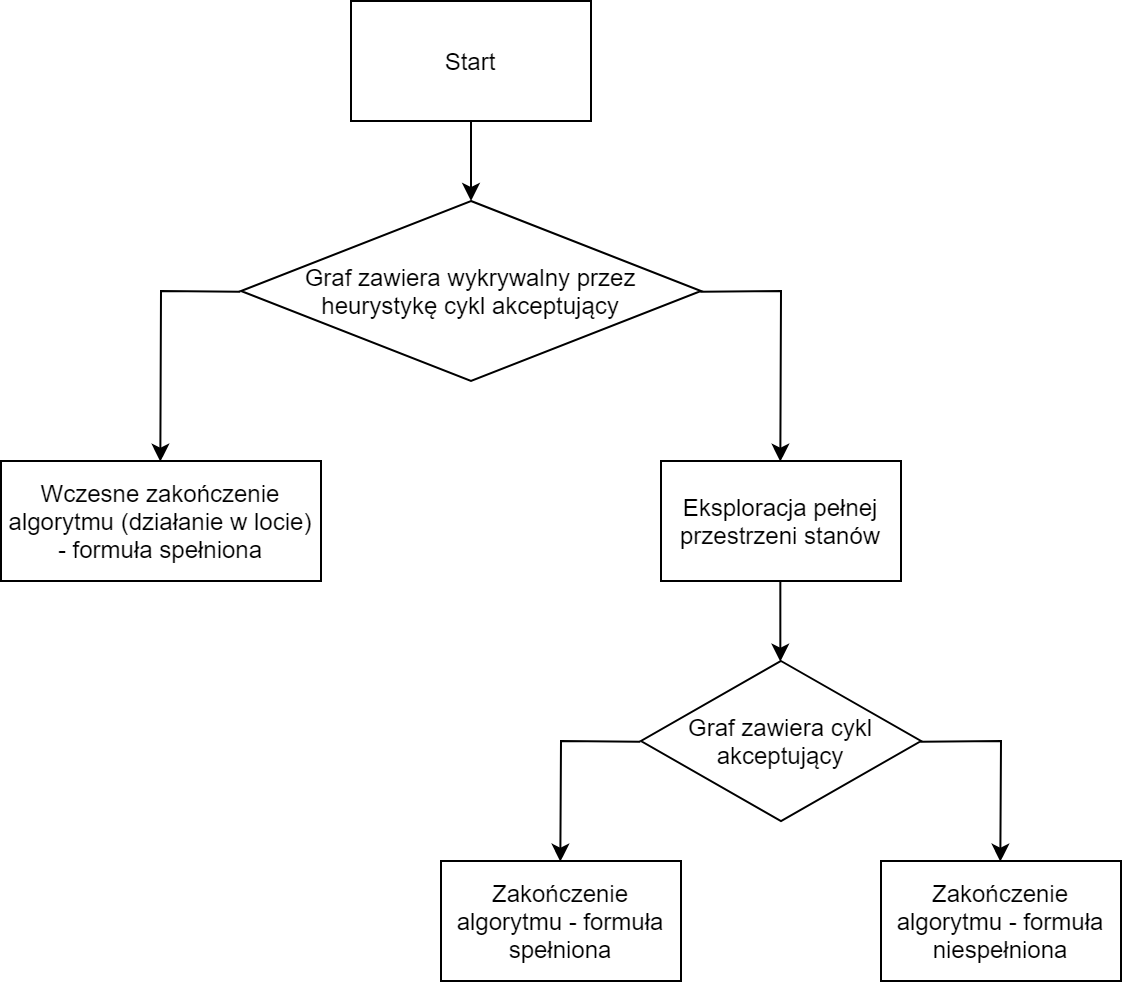
\includegraphics[height=11cm,keepaspectratio]{img/on-the-fly-diagram.png}
    \caption{Diagram prezentujący, kiedy dochodzi do wczesnego zakończenia algorytmu.}
    \label{fig:ltl_model_checking}
\end{figure}

\chapter{Prezentacja wyników}

\chapter{Podsumowanie}


\printbibliography

\end{document}
